% Options for packages loaded elsewhere
% Options for packages loaded elsewhere
\PassOptionsToPackage{unicode}{hyperref}
\PassOptionsToPackage{hyphens}{url}
\PassOptionsToPackage{dvipsnames,svgnames,x11names}{xcolor}
%
\documentclass[
  12pt,
  oneside]{book}
\usepackage{xcolor}
\usepackage[top=30mm,bottom=30mm,left=25mm,right=20mm,headheight=15mm,footskip=33pt]{geometry}
\usepackage{amsmath,amssymb}
\setcounter{secnumdepth}{5}
\usepackage{iftex}
\ifPDFTeX
  \usepackage[T1]{fontenc}
  \usepackage[utf8]{inputenc}
  \usepackage{textcomp} % provide euro and other symbols
\else % if luatex or xetex
  \usepackage{unicode-math} % this also loads fontspec
  \defaultfontfeatures{Scale=MatchLowercase}
  \defaultfontfeatures[\rmfamily]{Ligatures=TeX,Scale=1}
\fi
\usepackage{lmodern}
\ifPDFTeX\else
  % xetex/luatex font selection
\fi
% Use upquote if available, for straight quotes in verbatim environments
\IfFileExists{upquote.sty}{\usepackage{upquote}}{}
\IfFileExists{microtype.sty}{% use microtype if available
  \usepackage[]{microtype}
  \UseMicrotypeSet[protrusion]{basicmath} % disable protrusion for tt fonts
}{}
\usepackage{setspace}
\makeatletter
\@ifundefined{KOMAClassName}{% if non-KOMA class
  \IfFileExists{parskip.sty}{%
    \usepackage{parskip}
  }{% else
    \setlength{\parindent}{0pt}
    \setlength{\parskip}{6pt plus 2pt minus 1pt}}
}{% if KOMA class
  \KOMAoptions{parskip=half}}
\makeatother
% Make \paragraph and \subparagraph free-standing
\makeatletter
\ifx\paragraph\undefined\else
  \let\oldparagraph\paragraph
  \renewcommand{\paragraph}{
    \@ifstar
      \xxxParagraphStar
      \xxxParagraphNoStar
  }
  \newcommand{\xxxParagraphStar}[1]{\oldparagraph*{#1}\mbox{}}
  \newcommand{\xxxParagraphNoStar}[1]{\oldparagraph{#1}\mbox{}}
\fi
\ifx\subparagraph\undefined\else
  \let\oldsubparagraph\subparagraph
  \renewcommand{\subparagraph}{
    \@ifstar
      \xxxSubParagraphStar
      \xxxSubParagraphNoStar
  }
  \newcommand{\xxxSubParagraphStar}[1]{\oldsubparagraph*{#1}\mbox{}}
  \newcommand{\xxxSubParagraphNoStar}[1]{\oldsubparagraph{#1}\mbox{}}
\fi
\makeatother


\usepackage{longtable,booktabs,array}
\newcounter{none} % for unnumbered tables
\usepackage{calc} % for calculating minipage widths
% Correct order of tables after \paragraph or \subparagraph
\usepackage{etoolbox}
\makeatletter
\patchcmd\longtable{\par}{\if@noskipsec\mbox{}\fi\par}{}{}
\makeatother
% Allow footnotes in longtable head/foot
\IfFileExists{footnotehyper.sty}{\usepackage{footnotehyper}}{\usepackage{footnote}}
\makesavenoteenv{longtable}
\usepackage{graphicx}
\makeatletter
\newsavebox\pandoc@box
\newcommand*\pandocbounded[1]{% scales image to fit in text height/width
  \sbox\pandoc@box{#1}%
  \Gscale@div\@tempa{\textheight}{\dimexpr\ht\pandoc@box+\dp\pandoc@box\relax}%
  \Gscale@div\@tempb{\linewidth}{\wd\pandoc@box}%
  \ifdim\@tempb\p@<\@tempa\p@\let\@tempa\@tempb\fi% select the smaller of both
  \ifdim\@tempa\p@<\p@\scalebox{\@tempa}{\usebox\pandoc@box}%
  \else\usebox{\pandoc@box}%
  \fi%
}
% Set default figure placement to htbp
\def\fps@figure{htbp}
\makeatother





\setlength{\emergencystretch}{3em} % prevent overfull lines

\providecommand{\tightlist}{%
  \setlength{\itemsep}{0pt}\setlength{\parskip}{0pt}}



 


\usepackage{Archivo}
%\usepackage[sc]{mathpazo}

\usepackage[T1]{fontenc}
\usepackage{xcolor}
\usepackage[pages=some]{background}
\usepackage{setspace}
\usepackage[table]{xcolor}
\usepackage{tabularx}
\usepackage[Bjornstrup]{fncychap}
\usepackage{multirow}

% Colors Techtraplastice
\definecolor{Naranja}{HTML}{F69223}
\definecolor{Celeste}{HTML}{3299CC}
\definecolor{Verde}{HTML}{98C601}
\definecolor{Neutro}{HTML}{5E6F75}
\definecolor{Neutro_claro}{HTML}{F1F1F1}

\definecolor{Verde_osc}{RGB}{47,93,80}


% Headers
\usepackage{fancyhdr}
\pagestyle{fancy}          

\fancyhead{}
\fancyfoot{}

\fancyhead[L]{
\includegraphics[height=10mm]{assets/images/logo-TTPCE.png}}
\fancyhead[C]{ }
\fancyhead[R]{\thepage}

\fancyfoot[L]{
\includegraphics[height=8mm]{assets/images/footer-00.png}}
\fancyfoot[C]{}
\fancyfoot[R]{
\includegraphics[height=8mm]{assets/images/EU.png}}



\renewcommand{\headrulewidth}{1pt}
\renewcommand{\headruleskip}{1mm}



\usepackage{pdfpages}
\usepackage{wrapfig}
\usepackage{pgfgantt}
\usepackage{academicons}

\usepackage{worldflags}

% Command
\newcommand{\techtra}{\emph{TechTraPlastiCE }}

\usepackage{tabu}

% \usepackage{sectsty}
% \sectionfont{\scshape}
\usepackage{booktabs}
\usepackage{longtable}
\usepackage{array}
\usepackage{multirow}
\usepackage{wrapfig}
\usepackage{float}
\usepackage{colortbl}
\usepackage{pdflscape}
\usepackage{tabularx}
\usepackage{xltabular}
\usepackage{threeparttable}
\usepackage{threeparttablex}
\usepackage[normalem]{ulem}
\usepackage{makecell}
\usepackage{xcolor}
\makeatletter
\@ifpackageloaded{caption}{}{\usepackage{caption}}
\AtBeginDocument{%
\ifdefined\contentsname
  \renewcommand*\contentsname{Table of contents}
\else
  \newcommand\contentsname{Table of contents}
\fi
\ifdefined\listfigurename
  \renewcommand*\listfigurename{List of Figures}
\else
  \newcommand\listfigurename{List of Figures}
\fi
\ifdefined\listtablename
  \renewcommand*\listtablename{List of Tables}
\else
  \newcommand\listtablename{List of Tables}
\fi
\ifdefined\figurename
  \renewcommand*\figurename{Figure}
\else
  \newcommand\figurename{Figure}
\fi
\ifdefined\tablename
  \renewcommand*\tablename{Table}
\else
  \newcommand\tablename{Table}
\fi
}
\@ifpackageloaded{float}{}{\usepackage{float}}
\floatstyle{ruled}
\@ifundefined{c@chapter}{\newfloat{codelisting}{h}{lop}}{\newfloat{codelisting}{h}{lop}[chapter]}
\floatname{codelisting}{Listing}
\newcommand*\listoflistings{\listof{codelisting}{List of Listings}}
\makeatother
\makeatletter
\makeatother
\makeatletter
\@ifpackageloaded{caption}{}{\usepackage{caption}}
\@ifpackageloaded{subcaption}{}{\usepackage{subcaption}}
\makeatother
\usepackage{bookmark}
\IfFileExists{xurl.sty}{\usepackage{xurl}}{} % add URL line breaks if available
\urlstyle{same}
% fallback for those not using the hyperref driver hyperxmp:
\makeatletter
\@ifundefined{xmpquote}{\newcommand{\xmpquote}[1]{#1}}{}
\makeatother
\hypersetup{
  pdftitle={D5.2 Branding digital material and training program},
  pdfauthor={Lic. Marian Lenchours Pezzano ~; Mg. Marcos del Bello},
  colorlinks=true,
  linkcolor={Celeste},
  filecolor={Maroon},
  citecolor={Blue},
  urlcolor={Naranja},
  pdfcreator={LaTeX via pandoc}}


\title{D5.2 Branding digital material and training program}
\author{Lic. Marian Lenchours Pezzano ~ \and Mg. Marcos del Bello}
\date{November 25, 2026}
\begin{document}
  \begin{frontmatter}
  \begin{titlepage}
  % Inspiration: https://nmfs-opensci.github.io/quarto_titlepages_v1/02-titlepages.html
  % This is a combination of Pandoc templating and LaTeX
  % Pandoc templating https://pandoc.org/MANUAL.html#templates
  % See the README for help



  \backgroundsetup{
    scale=1.0,
    angle=0,
    opacity=0.90,
    contents={
      
\includegraphics{assets/Portada.png}}
      }

  \BgThispage


  \begin{minipage}[b][0.78\textheight][s]{0.65\textwidth}

    \raggedright
    % Title and subtitle
    
    \vfill

    \begin{spacing}{2.2}
      {\color{Naranja}\Huge\bfseries{D5.2 Branding digital material and
  training program}} \\[1\baselineskip] 
    \end{spacing}
    
    \begin{spacing}{1.2}
    {\color{Neutro} \Large\textit{WP5 -- Dissemination and
  Communication}}\\[1\baselineskip]
    
    {\Large \color{Neutro} 
    Strengthening University Tech Transfer Capabilities to Support Circular Economy 
    Value Chains for Plastics in Latin America -
    \textsc{\centering\bfseries TechTraPlastiCE} }\\[2\baselineskip]

    
    \end{spacing}

    {\color{Neutro} \Large\textit{November 25, 2026}}
    
    \vfill
  \end{minipage}		

  \vfill

  {\scriptsize
    \color{Neutro}
    This project has been funded with the support of Erasmus +.  
    The contents are the responsibility of the author(s). 
    The Commission cannot be held responsible for any use which may be made of the information contained therein. 
    Project No. 101179564 
    }


  \newpage



  \thispagestyle{plain}
  \begin{tabu} to \linewidth {X[1.3,l]  | X[1,l] X[1,l]}
    \toprule
    \multirow{5}{*}{ 
\includegraphics[height=20mm]{assets/images/logo-TTPCE.png}} &  \textbf{Work Package} : & WP5  \\ \cmidrule{2-3}
      & \textbf{Project Number} : & 101179564  \\ \cmidrule{2-3}
      &  \textbf{Type of document}:  & Deliverable   \\ \cmidrule{2-3}
      & \textbf{Due Delivery Date}:    & April
  30/2025     \\ \cmidrule{2-3}
      & \textbf{Actual Delivery Date}:    & November 25, 2026       \\ 
    \bottomrule
  \end{tabu}

  \vfill


  \begin{tabu} to \linewidth {X[1,l]  | X[3.5,l]}
    \toprule
    \textbf{Title} : & D5.2 Branding digital material and training
  program  \\ \cmidrule{2-2}
    \textbf{Work Package} : & WP5 -- Dissemination and
  Communication  \\ \cmidrule{2-2}
    \textbf{Description} : & The digital toolbox will contain all
  graphical material for branding and communication and the
  recommendations for usage. This will also be uploaded visible on the
  website. The recordings of the training - sessions will be
  available.  \\ \cmidrule{2-2}
    \textbf{Responsible} : & Universidad Nacional de Río
  Negro  \\ \cmidrule{2-2}
    \textbf{Author(s)} : &  
     
          Lic. Marian Lenchours Pezzano ~
          
          Mg. Marcos del Bello
           \\ \cmidrule{2-2}
    \textbf{Project Call} : & ERASMUS-EDU-2024-CBHE (Capacity building in the field of higher education)  \\ \cmidrule{2-2}
    \textbf{Dissemination Level} : & Confidential\\   
  \bottomrule
  \end{tabu}



  \vfill


  \begin{tabular}{ >{\raggedright\arraybackslash}p{3cm}| p{2cm} p{4cm} p{6cm} }
    \toprule
    \textbf{Version}: & \multicolumn{3}{l}{ 1.2} \\ \midrule
    \textbf{Contributors}  & Versions    & Dates       & Revision Description \\ \midrule
    WP5 Leader  & 1    & April 25/2025  & Global structure  \\ 
    Coordinator  & 1.1    & April 28/2025  & Validation of the global structure  \\ 
    USACH  & 1.2   & April 30/2025  & Validation  \\ 
    \bottomrule
\end{tabular}  


    
    
    \vfill
    
    {\scriptsize\centering\color{lightgray} 
    
    Disclaimer
    
    This document is provided <<as is>> with no warranties whatsoever, 
    including any warranty or merchantability, non-infringement, fitness for any particular 
    purpose, or any warranty otherwise arising out of any proposal, specification or sample.  
    
    No license, express or implied, by estoppels or otherwise, to any intellectual 
    property rights are granted herein. 
    The members of the project TechTraPlastiCE do not accept any liability for actions or 
    omissions of TechTraPlastiCE members or third parties and disclaim any obligation 
    to enforce the use of this document. 
    
    This document reflects only the authors' view and the Commission is not responsible 
    for any use that may be made of the information it contains.  
    This document is subject to change without notice. 
    
    }
    \normalsize
    
    
    
      \end{titlepage}
  \end{frontmatter}

\renewcommand*\contentsname{Contents}
{
\setcounter{tocdepth}{2}
\tableofcontents
}

\setstretch{1.2}
\mainmatter
\chapter{Executive summary}\label{executive-summary}

A logo and visual identity plan of the project, layout for
presentations, documents and other dissemination materials were created
in the first three months of the project (February 2025).

\textbf{All main dissemination materials will be provided in English and
Spanish to broaden the reach of all project results and impact the
target groups in the Latin America region}. It is essential to respect
the visual identity of the project in order to communicate it with
coherence and consistency.

Considering that communication is a dynamic process, WP5´s leader will
provide support in the communications and organization of events from
other WPs when it comes to dissemination tools and branding

\newpage

\section{Logos of the
TechTraplastiCE}\label{logos-of-the-techtraplastice}

WP5 leader, together with UL, participated in ideas generation
activities before the kick-off meeting (March 2025) and three proposals
of logo were designed and were submitted (via online) to all partners to
vote and express considerations.

In response to suggestions on the winning logo, a new version was
presented and approved by the consortium during the first Consortium
virtual meeting (28 February 2025).

Our logo is essential to our project It embodies our core proposition
and acts as a recognizable signature that unites all parts of
TechTraPlastiCE.

This TechTraPlastiCE logo also seeks to represent the principles of
circulareconomy, recycling, industry, academia and knowledge transfer.
Its design reflects the interconnection between academia, society and
industry to address the challenges of plastics and move towards a green
transition.

\section{UE Visibility}\label{ue-visibility}

The European Union (EU) has numerous funding programmes which support
projects and initiatives in various domains across the EU and beyond.
All beneficiaries, managing authorities and implementing partners of EU
funding must use the EU emblem in their communication to acknowledge the
support received under EU programmes and contribute to the visibility of
the EU on the ground.

Recipients of EU funding have a general obligation to communicate and
raise EU visibility. An important obligation in this context is the
correct and prominent display of the EU emblem, in combination with a
simple funding statement, mentioning the EU support.


\includepdf[landscape=false, delta=2 2, frame=true, 
pagecommand={\pagestyle{fancy}},
 nup=3x3, scale=0.8, offset=0 0cm, pages=-]{figures/5.2/00-logo-01.pdf}

\section{Branding manual}\label{branding-manual}

Based on the logo, a visual identity plan of the project was created in
the first three months of the project (February 2025).

This branding manual serves to define and guide the consistent
application of the visual elements of TechTraPlastiCE brand in any
context, ensuring a coherent and recognizable image.

It details how to use the logo, colors, typographies and other graphic
elements of the brand in different contexts, such as advertising, social
networks, web, stationery, etc. Following the guidelines in the manual
ensures that the brand has a consistent visual image, which facilitates
its recognition and improves its perception by the public.

The manual helps standardize brand creation and application processes,
reducing the time and effort required to maintain visual consistency. It
also serves as a reference tool for the internal team working with the
brand, ensuring that everyone follows the same guidelines. It can also
be useful for third parties working with the brand, such as advertising
agencies or designers, so that they can create materials consistent with
the visual identity.


\includepdf[landscape=false, delta=2 2, frame=true,  
scale=0.8, offset=0 0cm, pagecommand={\pagestyle{fancy}},
nup=2x4,pages=-]{figures/5.2/01-marca.pdf}

\section{Templates of Slides PPT}\label{templates-of-slides-ppt}

PPT presentations are widely used in international events and in
internal and external meetings of projects such as ours.

In this sense, they are a letter of introduction to our target
audiences. That is why the presentations in the framework of
TechTraplastiCE must respect the visual identity of the project.

These templates and the resources developed to meet the needs of each
presentation, seek to unify the image to communicate with greater
coherence and consistency.

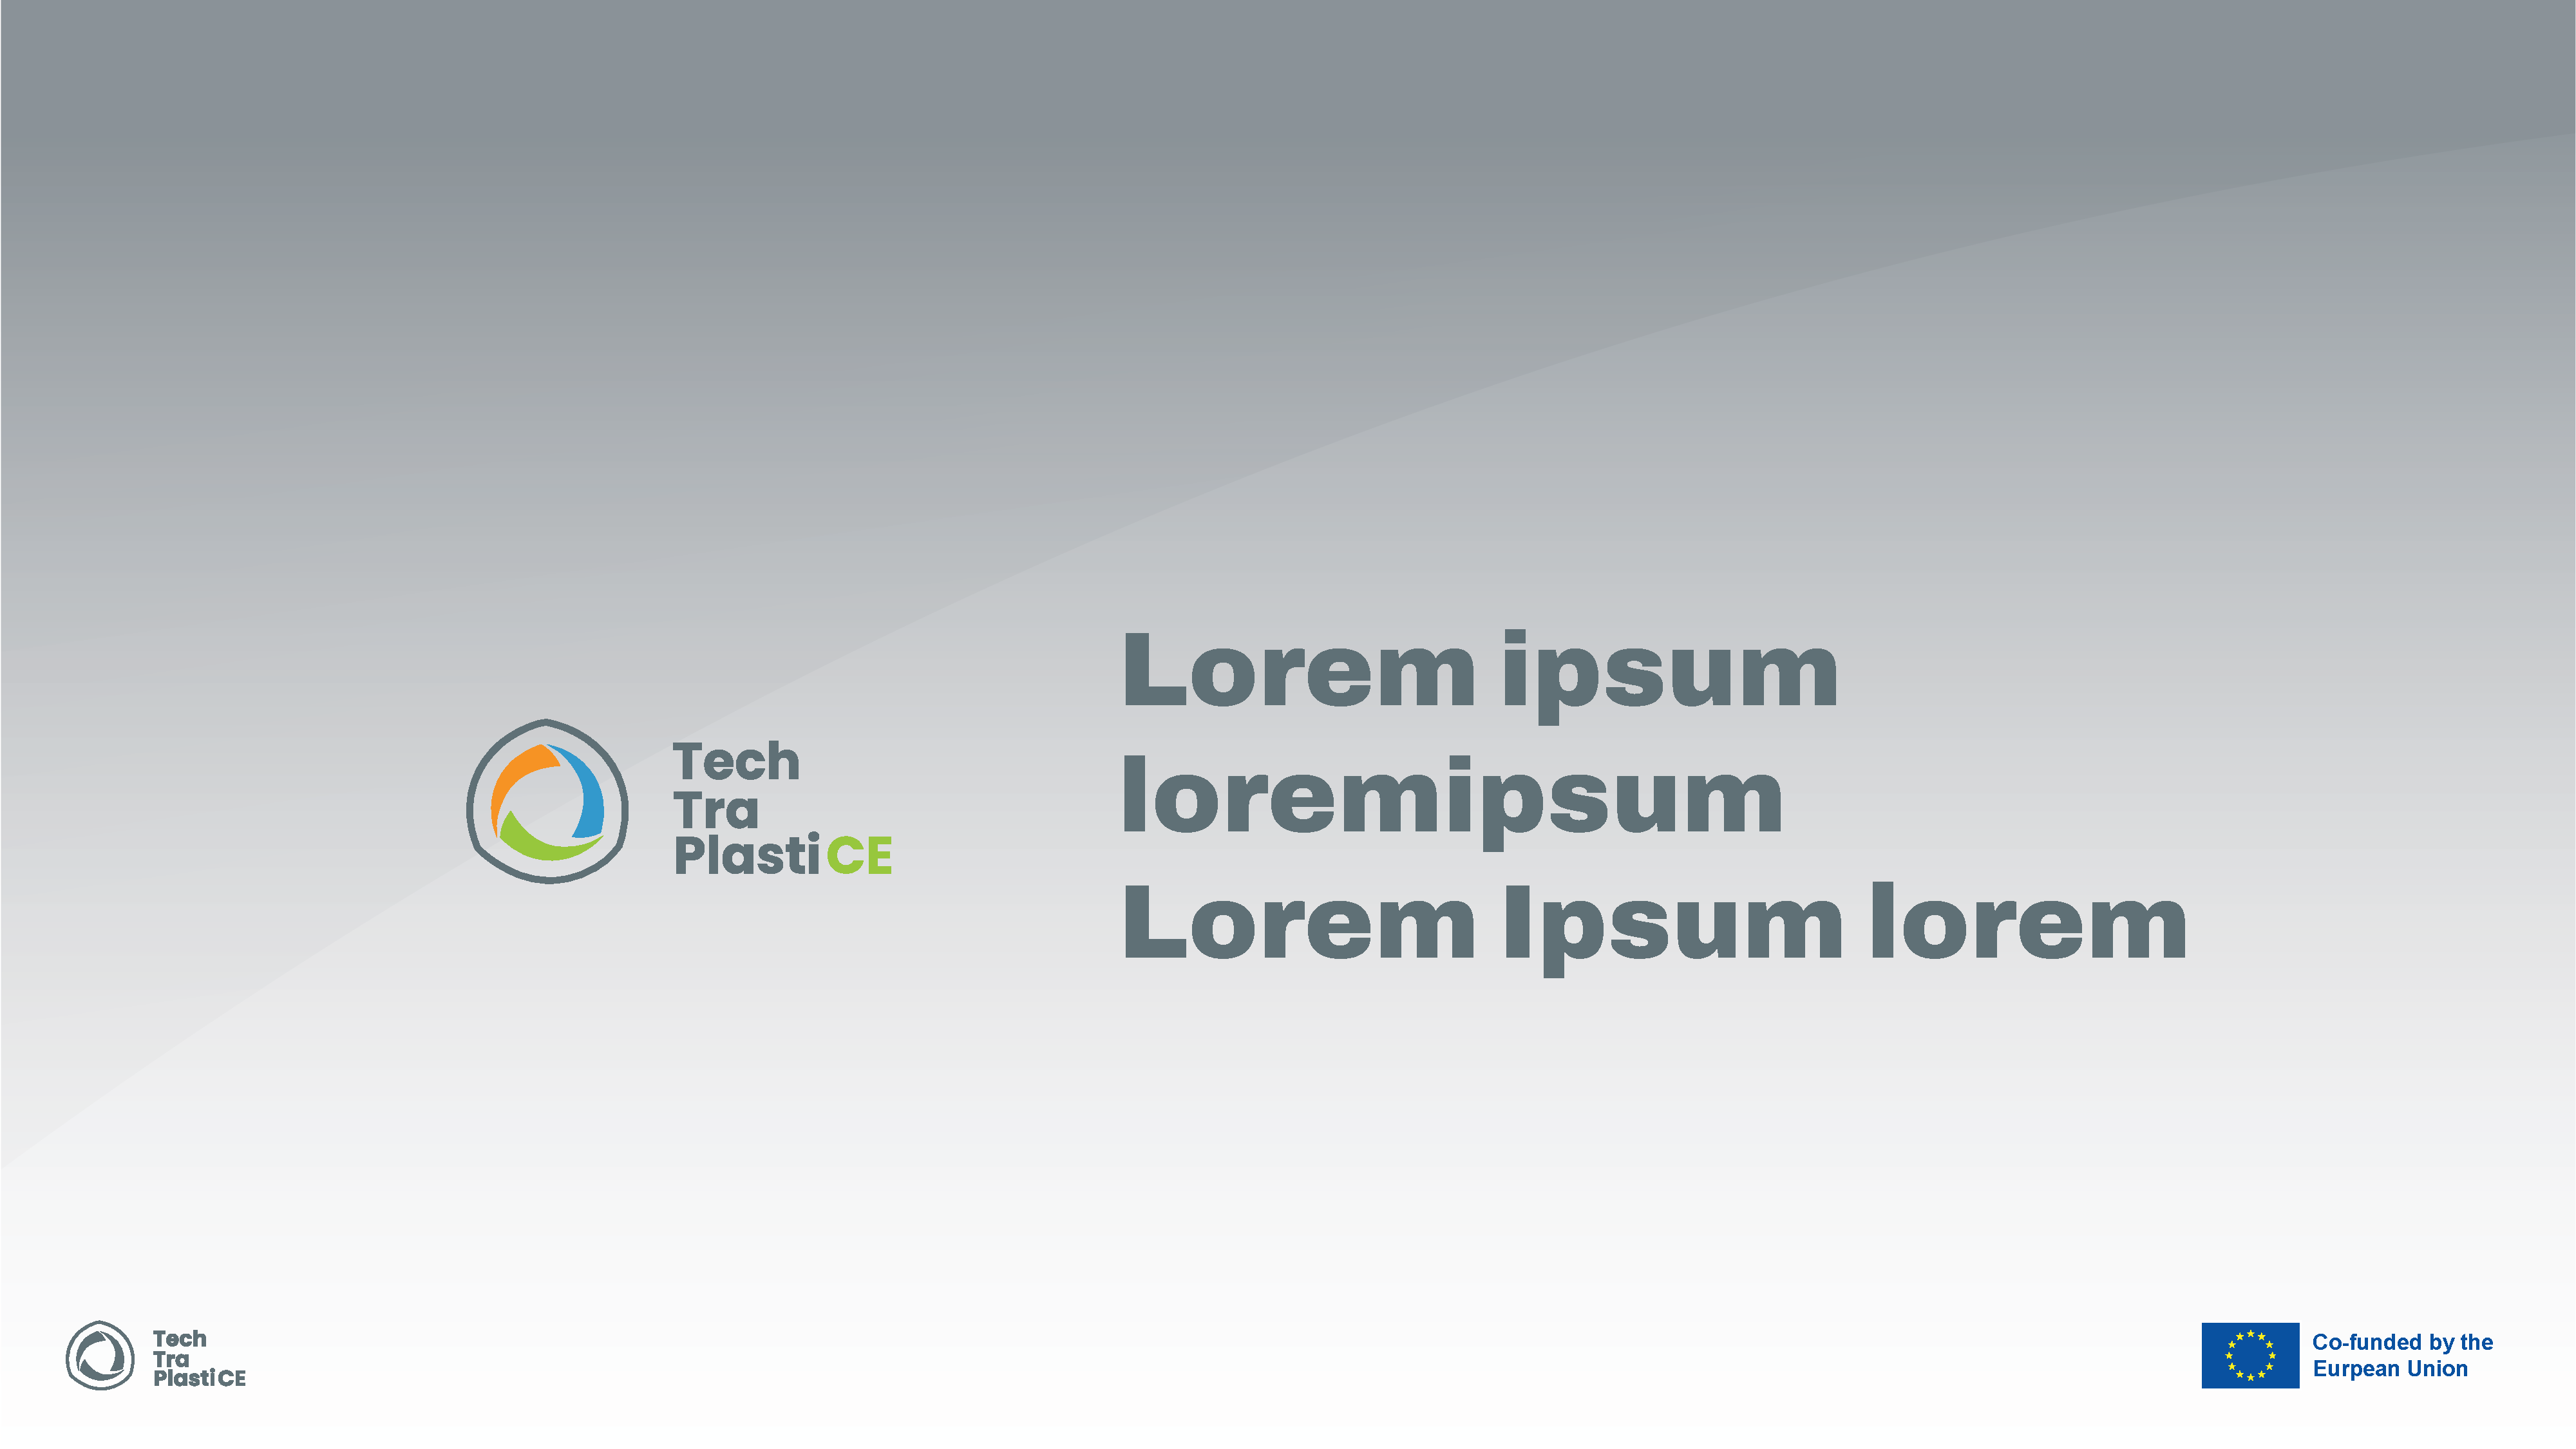
\includepdf[landscape=false, scale=0.8, offset=0 0cm,
pagecommand={\pagestyle{fancy}},
delta=2 2, frame=true,  nup=2x4,pages=-]{figures/5.2/03-Templates-ppt.pdf}

\section{Templates for media}\label{templates-for-media}

Based on the Brand Manual, the necessary resources were created to
create the project's profiles in social networks according to the
project's visual identity. This was applied to LinkedIn\footnote{See
  \url{https://www.linkedin.com/company/techtraplastice/?viewAsMember=true}}
as illustrated in Figure~\ref{fig-linkedin}, active since February 2025,
and will be applied to the project's accounts on X and YouTube, which
will be registered in May 2025.

In turn, templates will be designed for the creation of content in
social networks: ephemerides, infographics and promotional and
informative flyers.

\begin{figure}[H]

\centering{


\includegraphics[width=0.7\linewidth,height=\textheight,keepaspectratio]{figures/5.2/linkedin.png}

}

\caption{\label{fig-linkedin}\href{https://www.linkedin.com/company/techtraplastice/?viewAsMember=true}{Linkedin
account of the TechTraplastiCE.}}

\end{figure}%

\includepdf[landscape=false, delta=2 2, frame=true,  nup=2x3,
scale=0.8, offset=0 0cm, pagecommand={\pagestyle{fancy}},
pages=-]{figures/5.2/04-fotos.pdf}


\includepdf[landscape=false, delta=2 2, frame=true,  nup=3x3,
scale=0.8, offset=0 -3cm, 
pagecommand={\section{Templates for documents} All TechTraPlastiCE deliverables and documents developed under the project shall apply the following templates with the visual identity of the project.
}, 
pages=-]{figures/5.2/05-word.pdf}

\section{Templates for Video
materials}\label{templates-for-video-materials}

All TechTraPlastiCE graphic design and video pieces shared through the
project's communication channels or other channels must respect the
visual identity of the project.

While the visual identity is maintained, the design will be adapted to
each communication objective and content.

\includepdf[landscape=false, delta=2 2, frame=true,  nup=3x3,
pagecommand=\section{Vertical format}, pagecommand={\pagestyle{fancy}},
offset=0 -120,
pages=-]{figures/5.2/06-video.pdf}

\includepdf[landscape=false,  delta=2 2, frame=true,  nup=2x3, pagecommand={\pagestyle{fancy} \section{Horizontal format}}, 
scale=0.8, pages=-]{figures/5.2/06-video-horizontal.pdf}

\section{Others ressources}\label{others-ressources}

TechTraPlastiCE's digital and printed brochure, the digital newsletter
for the project's target audiences and all other necessary dissemination
materials will be designed in accordance with the project identity
manual.


\backmatter


\end{document}
